\chapter{Practical procedures in computing paths}\label{chap4} %%% chap 4

\section{Introduction}\pageoriginale\label{chap4-sec4.1}  %sec 4.1

We will consider the problem either in uniform
formulation \eqref{chap4-sec4.1-eq4.1a} or in
formulation \eqref{chap4-sec4.1-eq4.1b}:   
\begin{gather*}
G(x) = p \text{ where } G: \mathbb{R}^{N+1} \to \mathbb{R}^N;
\tag{4.1a}\label{chap4-sec4.1-eq4.1a} \\
G(u, \lambda )=P \text{ where, } G:\mathbb{R}^N \times \mathbb{R} \to
\mathbb{R}^N . \tag{4.1b}\label{chap4-sec4.1-eq4.1b} 
\end{gather*}

\begin{defi*}
\begin{enumerate}[(a)]
\item A path $\Gamma = \{ x(s):x(s)\in \Omega ,G(x(s)) = p$
  for all $s \in I \}$ is said to
  be regular if Rank $G_x(x(s)) = N$ for all $s \varepsilon I(\Omega
  \subset \mathbb{R}^{N+1})$. 

\item A path $\Gamma =\{ (u(s),\lambda (s)):u(s) \in \Omega, G
  (u(s), \lambda (s)) = p$ for all $ s \in I \}$ is regular if
  Rank $[G_u(s),G_ \lambda (s)] = N$ for all $s \in I (\bar{\lambda}
  \subset \mathbb{R}^N)$. 
\end{enumerate}
\end{defi*}

\setcounter{chaplemma}{1}
\begin{chaplemma}\label{chap4-lem4.2}
$\Rank [G_u,G_\lambda ] = N$ if and only if either
\begin{equation*}
\begin{array}{r@{\;\;}l}
\text{\rm(i)} & G_u  \text{ is nonsingular,}\\
\end{array}\tag{4.2}\label{chap4-eq4.2}
\end{equation*}
or
\begin{equation*}
\begin{array}{r@{\;\;}l}
\text{\rm(ii)} & \text{\rm(a)}~\dim N (g_u) = 1,\\  
            & \text{\rm(b)}~G_\lambda \notin  \Range
(G_u)\equiv R(G_u). 
\end{array}\tag{4.2}\label{chap4-addeq4.2}
\end{equation*}
\end{chaplemma}

\begin{proof}
If (i) is true, then Rank $[G_\lambda ,G_\lambda]=N$.  In the other
case, $G_\lambda$ is not a linear combination of columns of $G_u$  and
since $N(G_u)$ has dimension $1,(N-1)$ columns of $G_u$ are linearly
independent and hence $N$ columns\pageoriginale of $[G_u, G_\lambda]$
are linearly independent. 

Conversely, let Rank $[G_u,G_ \lambda ] = N$. Then either (i) holds or
not. If it does we are done. If not, then $\dim N(G_u) = 1$ or else we
cannot have Rank $[G_u,G_ \lambda] = N$. But then we must also have
$G_ \lambda \not\varepsilon R(G_u)$. Hence the lemma 
\end{proof}

\begin{chaplemma}\label{chap4-lem4.3}%4.3
Let $\Gamma$ be a regular path of \eqref{chap4-sec4.1-eq4.1a}. Then
there exists 
  an open tube $T_\Gamma \subset \Omega$ such that $p$ is a regular
  value for $G$ on $T_\Gamma$ and $\Gamma \subset T_\Gamma$. 
\end{chaplemma}

\begin{proof} 
Take any  point $x \in \Gamma$, then there exists a minor
matrix of rank $N$, say $M(x)$ of $G_x(x(s))$, such that $\det M(x)
\neq 0$. Recall that 
$$
\det M(x) = \prod \limits^{N}_{j=1} k_j(s)
$$
where $\{ k_j(s)\}$ are all ten eigenvalues of the matrix $M(x)$. Also
$\{ k_j(s)\}$ are smooth functions and $k_j(s)\neq 0$ for $j=1, \ldots
N$. Hence there will exists a neighbourhood of $x(s)$ in which the
eigenvalues do not vanish. Therefore in this neighbourhood, the minor
is nonvanishing. Such neighbourhoods exist at each point on $\Gamma$
and so the tube $T_\Gamma$ can be constructed 
\end{proof}

\begin{defi*}
A point $(u(s), \lambda (s))$ on $\Gamma$ is said to be simple limit
point (or  simple fold) if (ii a,b) of lemma \ref{chap4-lem4.2} holds. 
 \end{defi*} 
 
 We have on $\Gamma$:
\begin{equation*}
G(u(s), \lambda (s))-p = 0, \tag{4.4a}\label{chap4-eq4.4a}
\end{equation*}\pageoriginale 
so that:
\begin{equation*}
G_u(s)\dot{u}(s) +  G_\lambda (s)\dot{\lambda} (s) =
0. \tag{4.4b}\label{chap4-eq4.4b} 
\end{equation*} 
 
Note that at a fold point $s = s^0$, $\dot{\lambda} (s^0) = 0$
because 
$$
G_\lambda (s^0) \notin R(G_u(s^0)).
$$
 
 Hence $\dot{u}(s^0) \in N(G_u(s^0))$ at a fold point. Since $\dim
 N(G^0_u)=1$ at simple fold point $(u^0,\lambda^0)$, we can take: 
$$
 N(G^0_u)= \text{ span } \{ \phi \},
$$
and
$$
N(G^{oT}_u)= \text{ span } \{ \psi\}. 
$$
 
From \eqref{chap4-eq4.4b} we have:
$$
G_u^0 \ddot{u} +G_\lambda^0 \ddot{\lambda}^0 +G_{uu}^0 \dot{u}^0 
\dot{u}^0 +2 G^0_{u \lambda} \dot{u}^0 \dot{\lambda}^0 + G_{\lambda
 \lambda}^0\dot{\lambda}^0 \dot{\lambda}^0 = 0. 
$$
 
Multiplying throughout by $\psi^{T}$ and using the fact that $\xi \in
R(G_u^0)$ if and only if $\psi^{T} \xi=0$, we get: 
$$
\psi^{T} G^0_\lambda \ddot{\lambda}^0 + \psi^{T} G_{uu}^0 \dot{u}^0
\dot{u}^0=0,  
$$
as $\dot{\lambda} (s_0) = 0$ at a fold point. Since $G_\lambda^0
\notin  R(G^0_u)$, we have: 
$$
\psi^T G^0_\lambda \neq 0,
$$
and so 
$$
\ddot{\lambda} (s^0)= \frac{-\psi^T G^0_{uu}\dot{u}^0 \dot{u}^0}
      {\psi^T G^0_\lambda}. 
$$

But\pageoriginale $\dot{u} (s^0)=\alpha \phi$ for some scalar
$\alpha$. Hence:  
$$
\ddot{\lambda} (s^0) = - \alpha^2 \frac{-\psi^T G^0_{uu}\phi
\phi}{\psi^T G^0_ \lambda} . 
$$
 
If $\dfrac{-\psi^T G^0_{uu}\phi \phi}{\psi^T G^0_ \lambda} \neq 0$,
then we say that $(u^0,\lambda^0)$ is a simple quadratic fold. We
similarly define a `fold of order $m$' if $\lambda ^{(k)} (s^0) = 0$
for all $k=1, \ldots m-1$ and $\lambda ^{m}(s^0) \neq 0$. 

Usual methods of computing paths fail at a fold point. So in this
section we present an algorithm for computing paths, that does not
fail at simple fold point. 
 
\setcounter{section}{4}
\section{Pseudoarclength Continuation}\label{chap4-sec4.5}%sec 4.5

  We already mentioned that at fold points on a regular path, Newton's
 method fails during natural parameter continuation. The main idea in
 pseudoarclength continuation is to drop the natural parametrization
 by $\lambda$ and use some other parameterization. Consider the
 equation: 
 \begin{equation*}
G(u, \lambda ) = 0, \tag{4.6}\label{chap4-eq4.6}
 \end{equation*} 
where $G : \mathbb{R}^N \times \mathbb{R} \to \mathbb{R}^N$. If
$(u^0, \lambda^0)$ is any point on a regular path and
$(\dot{u},\dot{\lambda}^0)$ is the unit tangent to the path, then we
adjoin to \eqref{chap4-eq4.6} the scalar normalization: 
\begin{equation*}
N(u, \lambda , \Delta s) \equiv \dot{u}^{0^T}(u-u^0)+\dot{\lambda}^0
(\lambda  - \lambda^0 )- \Delta S = 0  \tag{4.7}\label{chap4-eq4.7} 
\end{equation*}
 
 This is the equation of a plane, which is perpendicular to the
 tangent $(\dot{u}^0, \dot{\lambda}^0)$ at a distance $\Delta s$ from
 $(u^0, \lambda^0)$ (see Fig.~\ref{chap4-fig4.1}). 
This plane will intersect the
curve $\Gamma$ if $\Delta s$  and the curvature of $\Gamma$ are
not\pageoriginale too large. That is we solve (4.6) and (4.7)
simultaneously for $(u(s), \lambda (s))$. Using Newton's method this
leads to the linear system: 
\begin{equation*}
\begin{bmatrix}
G^U_u \;\; G^U_\lambda \\ 
\dot{u}^{o^T} \;\; \dot{\lambda}^0
\end{bmatrix}
\begin{bmatrix}
\Delta u^U\\ \Delta \lambda ^U
\end{bmatrix}
=  - 
\begin{bmatrix}
G^U\\ N^U
\end{bmatrix} \tag{4.8}\label{chap4-eq4.8}
\end{equation*}
 
Here $G^U_u = G_u (u^U, \lambda^U)$, $G^U_\lambda = G_\lambda (u^U,
\lambda^U)$, and the iterates are $u^{U+1} = u^U + \Delta u^U$ and
$\lambda^{U+1} = \lambda^U + \Delta \lambda^U$. 
\begin{figure}[H]
\centering
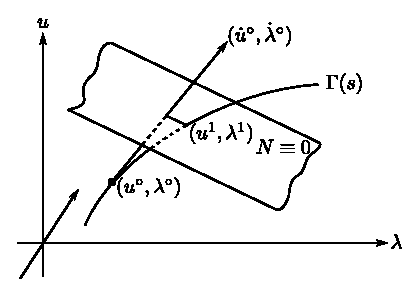
\includegraphics{vol79-fig/fig79-24.eps}
\smallskip
\caption{}
\label{chap4-fig4.1}
\end{figure}

We will give practical procedures for solving the system
\eqref{chap4-eq4.8} on a 
regular path. Recall that on such a path $G^0_u$ may be nonsingular
or singular but the $(N+1)$ order coefficient matrix should be
nonsingular. One proof of the nonsingular of the coefficient matrices
in \eqref{chap4-eq4.8} can be based on the following result (see:
\cite{key7}).  
 
\setcounter{chaplemma}{8}
\begin{chaplemma}\label{chap4-lem4.9} %4.9
Let\pageoriginale $B$ be a Banach space and let the linear operator
  $\tilde{A}: B \times \mathbb{R}^U \to B \times \mathbb{R}^U$ have
  the form: 
\begin{equation*}
\tilde{A} \equiv  
\begin{bmatrix}
A  & B \\ C^*  & D
\end{bmatrix},
\quad\text{where}\quad
\begin{cases}
A : B \to B, B : \mathbb{R}^U \to B, \\ 
C^* : B \to \mathbb{R}^U, D: \mathbb{R}^U \to \mathbb{R}^U.
\end{cases}
\end{equation*}   
\begin{enumerate}[\rm(i)]
\item If $A$ is nonsingular  then $\tilde{A}$ is nonsingular
  if and only if: 
\begin{equation*}
D - C^* A^{-1}B \text{ is nonsingular. } \tag{4.9a}\label{chap4-eq4.9a}
\end{equation*}

\item If $A$ is singular with
\begin{equation*}
\dim N(A)= \text{\rm\,Codim\,} R(A)=u, \tag{4.9b}\label{chap4-eq4.9b}
\end{equation*}
then $\tilde{A}$ is nonsingular if and only if:
\begin{equation*}
\begin{split}
(c_1) \dim R (B)& = u,  (c_2)R(B)\bigcap R(A)=0,\\
(c_3)\dim R (C^*)& = u, (c_4)N(A) \bigcap N(C^*) = 0. 
\end{split}\tag{4.9c}\label{chap4-eq4.9c}
\end{equation*}

\item If $A$ is singular with $\dim N(A) > u$, then
  $\tilde{A}$ is singular 
\end{enumerate} 
\end{chaplemma}

Here $C^*$ denotes the adjoin of $C$. In our analysis we use only the
cases $u = 1$ and $B \equiv \mathbb{R}^N$. Then the conditions
\eqref{chap4-eq4.9c} reduce to  
\begin{equation*}
B \notin R(A) \text{ and } C^T \notin
R(A^T). \tag{4.10}\label{chap4-eq4.10} 
\end{equation*}   
where $A^T$ is the transpose of $A$.

\begin{note*}
Instead of using the earlier mentioned normalization
\eqref{chap4-eq4.7}, we can  use other relation. One obvious
generalization of \eqref{chap4-eq4.7} is:  
$$
N \equiv \theta \dot{u}^{0^T}(u - u^0) + (1- \theta ) \lambda^0 (\lambda -
\lambda^0 ) - \Delta s = 0, 0 < \theta < 1; 
$$\pageoriginale

Another type of normalization is:
$$
N(u, \lambda, s) = \theta || u(s) - u(s^0) ||^2 + (1- \theta) |
\lambda (s) - \lambda (s^0) |^2 - (s - s^0)^2 = 0. 
$$

Alternatively if we know nearby point on $\Gamma$ say at $s = s_0$ and
$s = s_{-1}$ then we can use: 
\begin{align*}
N(u,\lambda, s) & = \theta \left[\frac{u(s_0) - u(s_{-1})}{s_0-s_{-1}}
  \right]^T
(u(s) - u(s_0))\\
& \qquad  + (1- \theta) \left[\frac{ \dot{\lambda} (s_0) - \dot{\lambda}
    (s_{-1})}{s_0 - s_{-1}} \right](\lambda (s) - \lambda (s_0)) - (s - s_0)
= 0. 
\end{align*}

This employs a scant rather a tangent. We call all of the above pseudo
arclength normalizations. For a references, see \cite{key18},
\cite{key19}.    
\end{note*}

\setcounter{section}{10}
\section{Bordering Algorithm}\label{chap4-sec4.11}%4.11

We write the coefficient matrix of \eqref{chap4-eq4.8} in the form:
\begin{equation*}
\tilde{A} = 
\begin{bmatrix}
A & b \\ c^T &  d ,
\end{bmatrix}\tag{4.12}\label{chap4-eq4.12}
\end{equation*}
where, $A$ is an $N \times N$ matrix, $b$, $c \in \mathbb{R}^N$
and $d \in \mathbb{R}$. Then we consider the linear system: 
\begin{equation*}
\tilde{A} \left(^{x}_\xi \right) = \left(^{g}_\gamma \right),
\tag{4.13}\label{chap4-eq4.13} 
\end{equation*} 
where $x$, $g \in \mathbb{R}^n$ and $\xi$, $\gamma \in
\mathbb{R}$. 

Assume $\tilde{A}$ and $A$ are nonsingular. Then solve the linear systems:
\begin{equation*}
Ay = b;\quad Az = g. \tag{4.14a}\label{chap4-eq4.14a}
\end{equation*} 

Form\pageoriginale the solution of \eqref{chap4-eq4.13} as:
\begin{equation*}
\xi = \frac{\gamma -c^{T_z}}{d-c^{T_y}}; x = z-\xi
y. \tag{4.14b}\label{chap4-eq4.14b} 
\end{equation*} 
 
Note that $d - c^Ty = d-c^T A^{-1}b$ is the Schur complement of $A$
 in $\tilde{A}$. Hence $d - c^Ty \neq 0$ if $\tilde{A}$
 nonsingular. Thus if $\tilde{A}$ and $A$ are nonsingular, then the
 bordering algorithm is valid. 
 
Alternatively we may also write the system \eqref{chap4-eq4.13} as:
\begin{align*}
Ax + b \xi &= g,\\
c^T x + d \xi &= \gamma .
\end{align*} 
 
To solve this, we can proceed by first eliminating $\xi$, if $d \neq
0$ to get:  
$$
\xi = \frac{1}{d}(\gamma - c^T x).
$$
 
Then for $x$ we have:
$$
(A - \frac{1}{d}bc^T ) x = g - \frac{\gamma}{d}b. 
$$
  
Note that $(A - \dfrac{1}{d}bc^T )$ is a rank 1 modification of
 $A$. Hence from the `Sherman-Morrison' formula (see lemma
\ref{chap2-sec2.29} in  Chapter \ref{chap2}), we can easily determine
the inverse of 
 $(A-\dfrac{1}{d}bc^T)$, once we know the inverse of $A$. In other
 words we can easily solve the linear system with the coefficient
 matrix $(A-\dfrac{1}{d}bc^T)$. But this procedure required $d \neq 0$
 while the bordering algorithm does not. The nonsingularity of $A$ is
 required by both. 
 
 Now we will consider the case when $A$ is singular and $\tilde{A}$ is
 nonsingular. This occurs at simple points on solution paths (see   
equation\pageoriginale (\ref{chap4-eq4.2},ii). That is we assume:
\begin{equation*}
\begin{array}{r@{\;\;}l}
\text{(i)} &  N(A)= \text{\ span\ } \{ \Phi\},\\
\text{(ii)} & b \notin R(A)\\
\text{(iii)} & c^T \notin R (A^T).
\end{array}\tag{4.15a}\label{chap4-eq4.15a}
\end{equation*}

These are precisely conditions \eqref{chap4-eq4.10} and are equivalent to:
\begin{equation*}
\psi ^T b  \neq o \text{ and } c^T \Phi \neq 0,
\tag{4.15b}\label{chap4-eq4.15b} 
\end{equation*}
where $\phi $ and $\psi$ are nontrivial solutions of :
\begin{equation*}
 A\phi = 0\quad \text{and}\quad A^T \psi =0.\tag
 {4.15c}\label{chap4-eq4.15c}  
\end{equation*}

We write the system \eqref{chap4-eq4.13} as :
$$
\widetilde {A}({^{X_{o}}_{\xi _{o}}})= (^g_\gamma), 
$$
where $x_0, g \in  \mathbb{R}^N$ and $\xi_0$, $U \in
\mathbb{R}$. That is: 
\begin{equation*}
\begin{split}
Ax_0 + b \xi_0 &= g,\\
c^T x_0 + d\xi _0& = \gamma, 
\end{split}\tag{4.16}\label{chap4-eq4.16}
\end{equation*}

Multiplying the first equation by $\psi ^T$, we get: 
\begin{equation*}
\xi _0 = \frac{\psi ^T g}{\psi ^T b}. \tag{4.17a}\label{chap4-eq4.17a}  
\end{equation*}

Hence 
\begin{equation*}
Ax_0 = g - \frac{\psi^T g}{\psi^T b} b \quad \in
R(A). \tag{4.17b}\label{chap4-eq4.17b}  
\end{equation*}

All solutions $x_0$ of \eqref{chap4-eq4.17b} have the form:
$$
x_0 = x_p + z \phi,
$$
where\pageoriginale $x_p$ is any particular solution of
\eqref{chap4-eq4.17b} and $z$ is 
obtained by substituting the value of $x_0$ into the second equation
of \eqref{chap4-eq4.16}  to get: 
$$
 z=\frac{\gamma - d \xi _0 - c^T x_p}{c^T \phi}. 
$$

Hence
\begin{equation*}
x_0= \left[x_p- \frac{c^T x_p}{c^T \phi }\phi  \right]+
\left(\frac{\gamma-d \xi 
  _0}{c^T \phi } \right)\phi. \tag{4.17c} \label{chap4-eq4.17c} 
\end{equation*}

Hence the unique solution of \eqref{chap4-eq4.16} is given  by
(\ref{chap4-eq4.17a},c). To 
evaluate this solution we need the  vectors $\phi$, $\psi$, $x_p$ and the
inner products $\psi^T g$, $\psi ^Tb$, $c^T \phi$ and $ c^T x_p$. 

The operational count to obtain these vectors is only one inner
product more than the count required by the Bordering Algorithm. Thus
the solution $( x_0, \xi_0)$ requires only two inner products more. We
will show how $\phi$ and $\psi$ can be obtained with half of a back
solve each and hence a total of one back solve.		 

\section*{Left and Right Null Vectors of A:}

Assume that  $A_1$ is an  $N \times N$ matrix satisfying
\eqref{chap4-eq4.15a} so 
that rank $(A_1)= N-1$. The with row and column interchanges
determined by some permutation matrices say, $P$ and $Q$, the
transformed matrix, 
\begin{equation*}
A \equiv PA_1Q, \tag{4.18a}\label{chap4-eq4.18a}
\end{equation*}
 has an $LU$ factorization:
 \begin{equation*}
	A= LU \equiv 
	\begin{bmatrix}
\hat{L} & 0\\
\hat{\ell}^T & 1 
	\end{bmatrix}
	\begin{bmatrix}
	\hat{U} & \hat{u}\\
	\hat{0}^T & 0
	\end{bmatrix} \tag{4.18b}\label{chap4-eq4.18b}
	\end{equation*}
	
Here\pageoriginale $\hat{L}$ and $\hat{U}$ are lower and upper
 triangular matrices, respectively, of order $(N-1)\times
 (N-1)$  with:  
$$
\hat{L}=
\begin{bmatrix}
1 & & & &  \\
\cdots & 1 & 0 & & \\
\cdots & \cdots & 1 & &\\
\cdots & \cdots & \cdots  & 1 & \\
\cdots &\cdots & \cdots & \cdots  & 1  
\end{bmatrix} \quad 
\hat{U}=
\begin{bmatrix}	
u_{11}& \cdots &\cdots & \cdots & \cdots \\
 & u_{22} & \cdots &\cdots & \cdots \\
  & 0 & \cdots & \cdots & \cdots \\
  & & & \cdots & \cdots\\
& & & & u_{N-1, N-1}
 \end{bmatrix}
 $$

Moreover: $ \hat{0}$, $\hat{u}$, $\hat{\ell} \in
\mathbb{R}^{N-1}$. Of course in actual calculations we do not get the
exact zero element in the final diagonal position of $U$. First we
discuss the null vectors and the  we will discuss the inexact
factorization.	 

Since $L$ is nonsingular, $A\phi =0 $ if and only if $U \phi =0 $. So
with $\hat{\phi} \in  \mathbb{R}^{N-1}$ and $  \alpha
\in  \mathbb{R}$, we seek $\phi $ in the form 
\begin{equation*}
\phi = \alpha \left(\displaystyle{\mathop{\hat{\phi}}_{-1}}
\right), \quad  \alpha \neq 0. \tag{4.19a}\label{chap4-eq4.19a} 
\end{equation*}

It follows because of the nonsingularity  of $\hat{U}$ that
$\hat{\phi}$ is uniquely determined by  
$$
\hat{U}\hat{\phi}= \hat{u}. 
$$

In other words:
$$
\hat{\phi}= \hat{U}^{-1}\hat{u}. 
$$

Since $U$ is  in triangular form, we obtain $\hat{\phi}$ and hence
$\phi$ with\pageoriginale only one half of a back solve (for a system
of order $N-1$). Similarly, the nonsingularity of $\hat{U}$ implies that
$A^T \psi = 0$ if and only if $L^T \psi = \beta
\left(\displaystyle{\mathop{\hat{0}}_{-1}} \right)$ 
for $\beta \in  \mathbb{R}$. Thus we find that all nontrivial
left null vectors are given by: 
\begin{equation*}
\psi = \left(\displaystyle{\mathop{\hat{\psi}}_{-1}} \right),
\quad \beta \neq 0, \tag{4.19b}\label{chap4-eq4.19b}
\end{equation*}
and $\hat{\psi} \in  \mathbb{R}^{N-1}$  is uniquely
determined by: 
\begin{align*}
\hat{L}^T \hat{\psi}&= \ell,\\
\hat{\psi} & = (\hat{L}^T)^{-1\hat{\ell}}.
\end{align*}

Again $\hat{\psi}$ and hence $\psi$ are obtained with half of a
back solve.  

\section*{Almost Singular A}%\sec

We already  mentioned that in calculations we do not obtain the exact
factorization, but  rather an approximation of the form: 
\begin{equation*}
A=A_\varepsilon  = L_\varepsilon  U_\varepsilon  = 
	\begin{pmatrix}
\hat{L}&\hat{o}\\
\hat{\ell}^T& 1
	\end{pmatrix}	
	\begin{pmatrix}
\hat{U}&\hat{u}\\
\hat{0}^T&\varepsilon  
	\end{pmatrix}.	 \tag{4.20}\label{chap4-eq4.20} 
\end{equation*}

The quantity $\varepsilon  $ will be an approximation to   zero. If we
use full pivoting to determine the permutation matrices $P$ and $Q$
in \eqref{chap4-eq4.18a}, then under appropriate conditions on $A_1$
we can bound 
$\varepsilon $ by $C10^{-t}$ for $t$ digit  arithmetic where $C$ is a
constant. The error analysis of Wilkinson \cite{key32} can also be used to
estimate the magnitude of $\varepsilon$. 

The basic assumptions that we make about the algorithm used to get the
form \eqref{chap4-eq4.20} and the error  growth allowed, are
summarized by the requirement that in the singular case
\eqref{chap4-eq4.15a}:  
$$
\max_{j<N} \left|\frac{\varepsilon }{u_{jj}}\right|\ll 1. 
$$

In\pageoriginale actual computations some precise relation must be
used if we are to 
declare that we are in the singular case. With partial pivoting in
columns, one reasonable test is: 
$$
\min_{j<N}\left|\frac{u_{jj}}{u_{j-1, j-1}}\right|> 10^2\left|
\frac{\varepsilon }{u_{N-1, N-1}}\right|. 
$$

Of course the factor $10^2$  may vary from case to case. A better
theory is needed here. 

Now we use the factorization \eqref{chap4-eq4.20} and apply the Bordering
Algorithm to solve \eqref{chap4-eq4.13}. So consider 
\begin{equation*}
a) \;  A_\varepsilon  y_\varepsilon  =b , \quad (b) \; A_\varepsilon  z_
\varepsilon  =g, \tag{4.21}\label{chap4-eq4.21} 
\end{equation*}
with 
$$
b= 
\begin{bmatrix}
\hat{b}\\
b_N 
\end{bmatrix}
, \quad g=
\begin{bmatrix}
\hat{g}\\
g_N
\end{bmatrix}.
$$

Now using $\phi $ and $\psi$ obtained from (\ref{chap4-eq4.19a},b)
with $ \alpha = \beta = 1$, we can easily see that: 
\begin{equation*}
\begin{split}
& \text{(a)} \; 	 y_\varepsilon =
\begin{bmatrix}
(\hat{L} \; \hat{U})^{-1} \hat{b}\\
0
\end{bmatrix}
+\frac{\psi ^T b}{\varepsilon } \phi\\
& \text{(b)} \;  z_\varepsilon =
\begin{bmatrix}
(\hat{L} \; \hat{U})^{-1}\hat{g}\\
0
\end{bmatrix}
+\frac{\psi ^T g}{\varepsilon }\phi 
\end{split}\tag{4.22}\label{chap4-eq4.22}
\end{equation*}

Now form (as in \eqref{chap4-eq4.14b})
\begin{equation*}
\begin{split}
& \text{(a)}   \; \xi_\varepsilon   = \frac{\gamma-\hat{c}^T
  (\hat{L} \, \hat{U})^{-1}\hat{g}- \frac{1}{\varepsilon
  }(\psi ^T g)(c^T \phi)}{d-\hat{c}^T
  (\hat{L} \, \hat{U})^{-1}\hat{b}- \frac{1}{\varepsilon }
  (\psi ^T b)(c^T \phi)},\\  
&\text{(b)} \;  x_\varepsilon   = 
\begin{bmatrix}
(\hat{L} \, \hat{U})^{-1}(\hat{g}- \xi _\varepsilon
  \hat{b})\\ 
0
\end{bmatrix}
+ \frac{1}{\varepsilon } [(\psi ^T g)- \xi _\varepsilon  (\psi ^T b)]
\phi . 
\end{split}\tag{4.23}\label{chap4-eq4.23}
\end{equation*}

 We\pageoriginale must compare the solution \eqref{chap4-eq4.23} with
 the exact  solution for the 
 singular case (\ref{chap4-eq4.17a},c). To do this, identify the
 particular  solution $x_p$ as:	 
 $$
  x_p \equiv
 \begin{bmatrix}
(\hat{L} \, \hat{U})^{-1}(\hat{g}- \xi _0 \hat{b})\\
0
\end{bmatrix}.
 $$
 
 Now we can expand \eqref{chap4-eq4.23} about $\varepsilon  = 0$ to
 obtain the results :  
  \begin{align*}
\xi_\varepsilon  & = \xi_0 + 0(\varepsilon),\\
x_\varepsilon  &= x_0 + 0 (\varepsilon).
 \end{align*} 
 
In more detail we have :
\begin{align*}
\xi_\varepsilon  & = \frac{ \varepsilon
  (\gamma-\hat{c}^T(\hat{L} \, \hat{U})^{-1}\hat{g} )-
  (\psi ^T g)(c^T \phi)}{\varepsilon
  (d-\hat{c}^T(\hat{L} \, \hat{U})^{-1}\hat{b})-( \psi ^T
  b) (c^T  \phi)},\\[3pt] 
  & = \frac{ \varepsilon
  (\gamma-\hat{c}^T(\hat{L} \, \hat{U})^{-1}\hat{g}
  )}{\varepsilon
  (d-\hat{c}^T(\hat{L} \, \hat{U})^{-1}\hat{b})-( \psi ^T
  b) (c^T  \phi)}\\
&\quad - \frac{  (\psi ^T g)(c^T \phi)}{\varepsilon
  (d-\hat{c}^T(\hat{L} \, \hat{U})^{-1}\hat{b})-( \psi ^T
  b) (c^T  \phi)},\\[3pt]  
 & =  \frac{\psi ^T g}{\psi ^T b}+ 0(\varepsilon ) = \xi _0 +0 (\xi).
 \end{align*} 

 Thus as $\varepsilon  \rightarrow 0$, the first term of the right
 hand side of (\ref{chap4-eq4.23}b) converges to $x_p$. Also : 
{\fontsize{10pt}{12pt}\selectfont
  \begin{align*}
\frac{1}{\varepsilon }[\psi ^T g- \xi (\psi ^Tb)]\phi
&=\frac{1}{\varepsilon } \left[ \frac{\psi ^T g.\varepsilon
    (d-\hat{c}^T(\hat{L}\hat{U}) ^{-1}\hat{b}) -
    \varepsilon  ( \gamma- \hat{c}^T
    (\hat{L}\hat{U})^{-1}\hat{g}) \psi ^T b}{\varepsilon
    (d-\hat{c}^T (\hat{L}\hat{U})^{-1}\hat{b})(\psi ^T
    b)(c ^T \phi)} \right] \phi\\[3pt] 
&=(\psi ^T b ) \frac{ \left[d. \frac{\psi ^T g}{\psi ^T b}- \gamma + c^T x_p
  \right] \phi}{\varepsilon \left[d-\hat{c}^T
    (\hat{L}\hat{U})^{-1}\hat{b} \right]- (\psi ^T b)(c ^T \phi
  )}\\[3pt] 
&= \frac{-d \xi _0 +\gamma - c^T x_p}{c^T \phi }\phi + 0 (\varepsilon
). 
 \end{align*}}\relax
 
Hence 
$$
x_\varepsilon  = x_0 +0 (\varepsilon ). 
$$
 
Note\pageoriginale that in the calculation the significant terms $\pm
(\psi ^T g)(\psi ^T b) (c^T \phi)$  cancelled each other. Here $\xi
_0, x_0$ are the exact exact solutions when $\varepsilon  = 0$. 
 
 Thus we find that the Bordering Algorithm can be used to solve
 \eqref{chap4-eq4.13} whenever $\widetilde {A}$ is nonsingular. If $A$
 happens to 
 be singular, then results of some accuracy will be obtained only if a
 reasonable  pivoting strategy is used. Even in this case some
 accuracy loss must be expected due to the  cancellation of significant
 digits that occurs in forming $x$ as in \eqref{chap4-eq4.14b}. 
 This cancellation
 is exactly analogous to the cancellation of the
 $\dfrac{1}{\varepsilon }$ terms in $x_\varepsilon  $ of
 (\ref{chap4-eq4.23}b). If 
 in the course of the calculations it is recognized that we are at a
 limit point then the singular $A$ algorithm can be used and a more
 accurate numerical solution  will result as no extra  significant
 digits are lost (see \cite{key17} for more details). We will give some
 numerical examples in the last chapter, in which we have used  the
 above algorithm and they have performed well.  


 \section*{The Tangent Vectors}
 
 We will briefly describe how to compute the tangent vectors
 $(\dot{u}^0$, $\dot{\lambda}^0)$. They must
 satisfy : 
\begin{equation*}
\begin{split}
& \text{(a)} \;  G^\circ_u \dot{u}^\circ + G^\circ_\lambda
\dot{\lambda}^\circ = 0,\\ 
& \text{(b)} \; || \dot{u}^\circ ||^2 + | \dot{\lambda}^\circ|^2 = 1. 
\end{split}\tag{4.24}\label{chap4-eq4.24}
\end{equation*}
 
First we consider regular points, where $G^\circ_u $ is
nonsingular. We find $\phi_0$. from: 
\begin{equation*}
 G_u^\circ \phi_0 = - G_\lambda^\circ. \tag{4.25}\label{chap4-eq4.25}
\end{equation*}

Then\pageoriginale set:
\begin{equation*}
\dot{u}^\circ = a \phi_0 \quad \text{and}  \quad \dot{\lambda}_0 = a
\tag{4.26}\label{chap4-eq4.26} 
\end{equation*} 
where $a$ is determined from (\ref{chap4-eq4.24}b) as :
\begin{equation*}
a=\frac{\pm 1}{\sqrt{1+|| \phi_0 ||^2}}. \tag{4.27}\label{chap4-eq4.27}
\end{equation*} 
 
The sign of a is chosen so that the orientation of the path is
preserved. More precisely, if $ (\dot{u}_{-1}, \dot{\lambda}_{-1})$
is the preceding tangent vector then we require 
$$
\dot{u}^T_{-1} \dot{u}^0 + \dot{\lambda}_{-1}
\dot{\lambda}^0> 0.  
$$
 
 Thus we choose the sign of `$a$' so that
 $$
 a[\dot{u}^{T}_{-1}\phi_0 + \dot{\lambda}_{-1}]>0. 
 $$

 Choosing the sign of a is very important in numerical
 calculations. If we do not choose the sign of a properly, either we
 will get trapped in the iterations at some point or it will reverse
 the direction and hence it will compute the same path already
 computed. 
 
 Another important point to recall in actual calculations  is that the
 quantity $||\dot {u}||^2$ is usually meant to approximate some $L_2$
 norm of the continuous formulation of the problem. Thus the net
 spacing, say $h$, must be used to form for example : 
$$
|| \dot{u}||^2 = \sum _{j=1}^J h^d \dot{u}_j^2. 
$$
 
Here $\dot{u}_j$ represent  the components of $\dot{u}$ and the
underlying continuous problem\pageoriginale is assumed formulated over
a domain in 
$\mathbb{R}^d$. If this is not done the arclength definition
$||\dot{u}||^2 + \dot{\lambda}^2$ is biased too much in the
$u$-subspace and $\lambda$ is not very significant. 
 
 We return to the case of a simple fold at which $G^\circ_u$
 is singular. The analysis of the case of almost singular $A$,
\eqref{chap4-eq4.20}--\eqref{chap4-eq4.22}, shows  that we get in this
case for the solution of 
\eqref{chap4-eq4.25}, by setting  
  \begin{equation*}
\phi_0 = 
\begin{bmatrix}
\hat {\phi}_0\\
\omega _0
\end{bmatrix}
, \quad -G^\circ_\lambda=
\begin{bmatrix}
\hat{g}\\
\gamma
\end{bmatrix} 
;\tag{4.28a}\label{chap4-eq4.28a}
 \end{equation*} 
 
 The result :
 \begin{equation*}
\begin{split}
& \hat{\phi}_0 = - (\hat{L} \, \hat{U}) ^{-1}\hat{g}+
\left(\frac{\gamma -\hat {\psi}^T \hat {g}}{\varepsilon } \right)
\hat {\phi},\\ 
& \omega_0 = - \left(\frac{\gamma- \hat{\psi}^T \hat{g}}{\varepsilon
 } \right) \equiv \frac{\beta}{\varepsilon }\quad  \text{(say)
 }. 
\end{split}\tag{4.28b}\label{chap4-eq4.28b} 
 \end{equation*}
 
Using these results (4.28) in \eqref{chap4-eq4.26} and
\eqref{chap4-eq4.27} we find that we 
 indeed get the tangent to within $0(\varepsilon)$. 
